%%%% Paramétrage du TD %%%%
\def\xxactivite{Synthèse 1 \ifprof -- Corrigé \else \fi} % \normalsize \vspace{-.4cm}
\def\xxauteur{\textsl{Xavier Pessoles}}

\def\xxnumchapitre{Chapitre 3 \vspace{.2cm}}
\def\xxchapitre{\hspace{.12cm} Application du Principe Fondamental de la Dynamique}

\def\xxtitreexo{Le robot humanoïde Lola}
\def\xxsourceexo{\hspace{.2cm} \footnotesize{Concours Mines Ponts -- PSI 2015}}
%\def\xxauteur{\textsl{Xavier Pessoles}}


\def\xxcompetences{%
\vspace{-.5cm}
\textsl{%
\textbf{Savoirs et compétences :}
\begin{itemize}[label=\ding{112},font=\color{ocre}] 
%\item \textit{Mod2.C16} : torseur cinétique
%\item \textit{Mod2.C17} : torseur dynamique
\item \textit{Mod2.C17.SF1} : déterminer le torseur dynamique d’un solide, ou d’un ensemble de solides, par rapport à un autre solide
%\item \textit{Mod2.C15} : matrice d'inertie
\item \textit{Res1.C2} : principe fondamental de la dynamique
%\item \textit{Res1.C1.SF1} : proposer une démarche permettant la détermination de la loi de mouvement
%\item \textit{Res1.C2.SF1} : proposer une méthode permettant la détermination d’une inconnue de liaison
\end{itemize}
}}
\def\xxfigures{
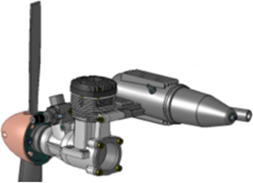
\includegraphics[width=.5\linewidth]{fig_00}}%figues de la page de garde


\iflivret
\pagestyle{empty}


%%%%%%%% PAGE DE GARDE COURS
\ifcours
% ==== BANDEAU DES TITRES ==== 
\begin{tikzpicture}[remember picture,overlay]
\node at (current page.north west)
{\begin{tikzpicture}[remember picture,overlay]
\node[anchor=north west,inner sep=0pt] at (0,0) {\includegraphics[width=\paperwidth]{\thechapterimage}};
\draw[anchor=west] (-2cm,-8cm) node [line width=2pt,rounded corners=15pt,draw=ocre,fill=white,fill opacity=0.6,inner sep=40pt]{\strut\makebox[22cm]{}};
\draw[anchor=west] (1cm,-8cm) node {\huge\sffamily\bfseries\color{black} %
\begin{minipage}{1cm}
\rotatebox{90}{\LARGE\sffamily\textsc{\color{ocre}\textbf{\xxnumpartie}}}
\end{minipage} \hfill
\begin{minipage}[c]{14cm}
\begin{titrepartie}
\begin{flushright}
\renewcommand{\baselinestretch}{1.1} 
\Large\sffamily\textsc{\textbf{\xxpartie}}
\renewcommand{\baselinestretch}{1} 
\end{flushright}
\end{titrepartie}
\end{minipage} \hfill
\begin{minipage}[c]{3.5cm}
{\large\sffamily\textsc{\textbf{\color{ocre} \discipline}}}
\end{minipage} 
 };
\end{tikzpicture}};
\end{tikzpicture}
% ==== FIN BANDEAU DES TITRES ==== 


% ==== ONGLET 
\begin{tikzpicture}[overlay]
\node[shape=rectangle, 
      rounded corners = .25 cm,
	  draw= ocre,
	  line width=2pt, 
	  fill = ocre!10,
	  minimum width  = 2.5cm,
	  minimum height = 3cm,] at (18.3cm,0) {};
\node at (17.7cm,0) {\rotatebox{90}{\textbf{\Large\color{ocre}{\classe}}}};
%{};
\end{tikzpicture}
% ==== FIN ONGLET 


\vspace{3.5cm}

\begin{tikzpicture}[remember picture,overlay]
\draw[anchor=west] (-2cm,-6cm) node {\huge\sffamily\bfseries\color{black} %
\begin{minipage}{2cm}
\begin{center}
\LARGE\sffamily\textsc{\color{ocre}\textbf{\xxactivite}}
\end{center}
\end{minipage} \hfill
\begin{minipage}[c]{15cm}
\begin{titrechapitre}
\renewcommand{\baselinestretch}{1.1} 
\Large\sffamily\textsc{\textbf{\xxnumchapitre}}

\Large\sffamily\textsc{\textbf{\xxchapitre}}
\vspace{.5cm}

\renewcommand{\baselinestretch}{1} 
\normalsize\normalfont
\xxcompetences
\end{titrechapitre}
\end{minipage}  };
\end{tikzpicture}
\vfill

\begin{flushright}
\begin{minipage}[c]{.3\linewidth}
\begin{center}
\xxfigures
\end{center}
\end{minipage}\hfill
\begin{minipage}[c]{.6\linewidth}
\startcontents
%\printcontents{}{1}{}
\printcontents{}{1}{}
\end{minipage}
\end{flushright}

\begin{tikzpicture}[remember picture,overlay]
\draw[anchor=west] (4.5cm,-.7cm) node {
\begin{minipage}[c]{.2\linewidth}
\begin{flushright}

\includegraphics[width=2cm]{logoCC}
\end{flushright}
\end{minipage}
\begin{minipage}[c]{.2\linewidth}
\textsl{\xxauteur} \\
\textsl{\classe}
\end{minipage}
 };
\end{tikzpicture}

\newpage
\pagestyle{fancy}

%\newpage
%\pagestyle{fancy}

\else
\fi
%% FIN PAGE DE GARDE DES COURS

%%%%%%%% PAGE DE GARDE TD
\iftd
%\begin{tikzpicture}[remember picture,overlay]
%\node at (current page.north west)
%{\begin{tikzpicture}[remember picture,overlay]
%\draw[anchor=west] (-2cm,-3.25cm) node [line width=2pt,rounded corners=15pt,draw=ocre,fill=white,fill opacity=0.6,inner sep=40pt]{\strut\makebox[22cm]{}};
%\draw[anchor=west] (1cm,-3.25cm) node {\huge\sffamily\bfseries\color{black} %
%\begin{minipage}{1cm}
%\rotatebox{90}{\LARGE\sffamily\textsc{\color{ocre}\textbf{\xxnumpartie}}}
%\end{minipage} \hfill
%\begin{minipage}[c]{13.5cm}
%\begin{titrepartie}
%\begin{flushright}
%\renewcommand{\baselinestretch}{1.1} 
%\Large\sffamily\textsc{\textbf{\xxpartie}}
%\renewcommand{\baselinestretch}{1} 
%\end{flushright}
%\end{titrepartie}
%\end{minipage} \hfill
%\begin{minipage}[c]{3.5cm}
%{\large\sffamily\textsc{\textbf{\color{ocre} \discipline}}}
%\end{minipage} 
% };
%\end{tikzpicture}};
%\end{tikzpicture}

%%%%%%%%%% PAGE DE GARDE TD %%%%%%%%%%%%%%%
%\begin{tikzpicture}[overlay]
%\node[shape=rectangle, 
%      rounded corners = .25 cm,
%	  draw= ocre,
%	  line width=2pt, 
%	  fill = ocre!10,
%	  minimum width  = 2.5cm,
%	  minimum height = 2.5cm,] at (18.5cm,0) {};
%\node at (17.7cm,0) {\rotatebox{90}{\textbf{\Large\color{ocre}{\classe}}}};
%%{};
%\end{tikzpicture}

% PARTIE ET CHAPITRE
%\begin{tikzpicture}[remember picture,overlay]
%\draw[anchor=west] (-1cm,-2.1cm) node {\large\sffamily\bfseries\color{black} %
%\begin{minipage}[c]{15cm}
%\begin{flushleft}
%\xxnumchapitre \\
%\xxchapitre
%\end{flushleft}
%\end{minipage}  };
%\end{tikzpicture}

% BANDEAU EXO
\iflivret % SI LIVRET
\begin{tikzpicture}[remember picture,overlay]
\draw[anchor=west] (-2cm,-3.3cm) node {\huge\sffamily\bfseries\color{black} %
\begin{minipage}{5cm}
\begin{center}
\LARGE\sffamily\color{ocre}\textbf{\textsc{\xxactivite}}

\begin{center}
\xxfigures
\end{center}

\end{center}
\end{minipage} \hfill
\begin{minipage}[c]{12cm}
\begin{titrechapitre}
\renewcommand{\baselinestretch}{1.1} 
\large\sffamily\textbf{\textsc{\xxtitreexo}}

\small\sffamily{\textbf{\textit{\color{black!70}\xxsourceexo}}}
\vspace{.5cm}

\renewcommand{\baselinestretch}{1} 
\normalsize\normalfont
\xxcompetences
\end{titrechapitre}
\end{minipage}};
\end{tikzpicture}
\else % ELSE NOT LIVRET
\begin{tikzpicture}[remember picture,overlay]
\draw[anchor=west] (-2cm,-4.5cm) node {\huge\sffamily\bfseries\color{black} %
\begin{minipage}{5cm}
\begin{center}
\LARGE\sffamily\color{ocre}\textbf{\textsc{\xxactivite}}

\begin{center}
\xxfigures
\end{center}

\end{center}
\end{minipage} \hfill
\begin{minipage}[c]{12cm}
\begin{titrechapitre}
\renewcommand{\baselinestretch}{1.1} 
\large\sffamily\textbf{\textsc{\xxtitreexo}}

\small\sffamily{\textbf{\textit{\color{black!70}\xxsourceexo}}}
\vspace{.5cm}

\renewcommand{\baselinestretch}{1} 
\normalsize\normalfont
\xxcompetences
\end{titrechapitre}
\end{minipage}};
\end{tikzpicture}

\fi

\else   % FIN IF TD
\fi


%%%%%%%% PAGE DE GARDE FICHE
\iffiche
\begin{tikzpicture}[remember picture,overlay]
\node at (current page.north west)
{\begin{tikzpicture}[remember picture,overlay]
\draw[anchor=west] (-2cm,-2.25cm) node [line width=2pt,rounded corners=15pt,draw=ocre,fill=white,fill opacity=0.6,inner sep=40pt]{\strut\makebox[22cm]{}};
\draw[anchor=west] (1cm,-2.25cm) node {\huge\sffamily\bfseries\color{black} %
\begin{minipage}{1cm}
\rotatebox{90}{\LARGE\sffamily\textsc{\color{ocre}\textbf{\xxnumpartie}}}
\end{minipage} \hfill
\begin{minipage}[c]{14cm}
\begin{titrepartie}
\begin{flushright}
\renewcommand{\baselinestretch}{1.1} 
\large\sffamily\textsc{\textbf{\xxpartie} \\} 

\vspace{.2cm}

\normalsize\sffamily\textsc{\textbf{\xxnumchapitre -- \xxchapitre}}
\renewcommand{\baselinestretch}{1} 
\end{flushright}
\end{titrepartie}
\end{minipage} \hfill
\begin{minipage}[c]{3.5cm}
{\large\sffamily\textsc{\textbf{\color{ocre} \discipline}}}
\end{minipage} 
 };
\end{tikzpicture}};
\end{tikzpicture}

\iflivret
\begin{tikzpicture}[overlay]
\node[shape=rectangle, 
      rounded corners = .25 cm,
	  draw= ocre,
	  line width=2pt, 
	  fill = ocre!10,
	  minimum width  = 2.5cm,
	  minimum height = 2.5cm,] at (18.5cm,.5cm) {};
\node at (17.9cm,.5cm) {\rotatebox{90}{\textsf{\textbf{\large\color{ocre}{\classe}}}}};
%{};
\end{tikzpicture}
\else
\begin{tikzpicture}[overlay]
\node[shape=rectangle, 
      rounded corners = .25 cm,
	  draw= ocre,
	  line width=2pt, 
	  fill = ocre!10,
	  minimum width  = 2.5cm,
%	  minimum height = 2.5cm,] at (18.5cm,1.1cm) {};
	  minimum height = 2.5cm,] at (18.6cm,0.5cm) {};
\node at (18cm,0.5cm) {\rotatebox{90}{\textsf{\textbf{\large\color{ocre}{\classe}}}}};
%{};
\end{tikzpicture}

\fi

\else
\fi



\else
\pagestyle{empty}


%%%%%%%% PAGE DE GARDE COURS
\ifcours
% ==== BANDEAU DES TITRES ==== 
\begin{tikzpicture}[remember picture,overlay]
\node at (current page.north west)
{\begin{tikzpicture}[remember picture,overlay]
\node[anchor=north west,inner sep=0pt] at (0,0) {\includegraphics[width=\paperwidth]{\thechapterimage}};
\draw[anchor=west] (-2cm,-8cm) node [line width=2pt,rounded corners=15pt,draw=ocre,fill=white,fill opacity=0.6,inner sep=40pt]{\strut\makebox[22cm]{}};
\draw[anchor=west] (1cm,-8cm) node {\huge\sffamily\bfseries\color{black} %
\begin{minipage}{1cm}
\rotatebox{90}{\LARGE\sffamily\textsc{\color{ocre}\textbf{\xxnumpartie}}}
\end{minipage} \hfill
\begin{minipage}[c]{14cm}
\begin{titrepartie}
\begin{flushright}
\renewcommand{\baselinestretch}{1.1} 
\Large\sffamily\textsc{\textbf{\xxpartie}}
\renewcommand{\baselinestretch}{1} 
\end{flushright}
\end{titrepartie}
\end{minipage} \hfill
\begin{minipage}[c]{3.5cm}
{\large\sffamily\textsc{\textbf{\color{ocre} \discipline}}}
\end{minipage} 
 };
\end{tikzpicture}};
\end{tikzpicture}
% ==== FIN BANDEAU DES TITRES ==== 


% ==== ONGLET 
\begin{tikzpicture}[overlay]
\node[shape=rectangle, 
      rounded corners = .25 cm,
	  draw= ocre,
	  line width=2pt, 
	  fill = ocre!10,
	  minimum width  = 2.5cm,
	  minimum height = 3cm,] at (18.3cm,0) {};
\node at (17.7cm,0) {\rotatebox{90}{\textbf{\Large\color{ocre}{\classe}}}};
%{};
\end{tikzpicture}
% ==== FIN ONGLET 


\vspace{3.5cm}

\begin{tikzpicture}[remember picture,overlay]
\draw[anchor=west] (-2cm,-6cm) node {\huge\sffamily\bfseries\color{black} %
\begin{minipage}{2cm}
\begin{center}
\LARGE\sffamily\textsc{\color{ocre}\textbf{\xxactivite}}
\end{center}
\end{minipage} \hfill
\begin{minipage}[c]{15cm}
\begin{titrechapitre}
\renewcommand{\baselinestretch}{1.1} 
\Large\sffamily\textsc{\textbf{\xxnumchapitre}}

\Large\sffamily\textsc{\textbf{\xxchapitre}}
\vspace{.5cm}

\renewcommand{\baselinestretch}{1} 
\normalsize\normalfont
\xxcompetences
\end{titrechapitre}
\end{minipage}  };
\end{tikzpicture}
\vfill

\begin{flushright}
\begin{minipage}[c]{.3\linewidth}
\begin{center}
\xxfigures
\end{center}
\end{minipage}\hfill
\begin{minipage}[c]{.6\linewidth}
\startcontents
%\printcontents{}{1}{}
\printcontents{}{1}{}
\end{minipage}
\end{flushright}

\begin{tikzpicture}[remember picture,overlay]
\draw[anchor=west] (4.5cm,-.7cm) node {
\begin{minipage}[c]{.2\linewidth}
\begin{flushright}

\includegraphics[width=2cm]{logoCC}
\end{flushright}
\end{minipage}
\begin{minipage}[c]{.2\linewidth}
\textsl{\xxauteur} \\
\textsl{\classe}
\end{minipage}
 };
\end{tikzpicture}

\newpage
\pagestyle{fancy}

%\newpage
%\pagestyle{fancy}

\else
\fi
%% FIN PAGE DE GARDE DES COURS

%%%%%%%% PAGE DE GARDE TD
\iftd
%\begin{tikzpicture}[remember picture,overlay]
%\node at (current page.north west)
%{\begin{tikzpicture}[remember picture,overlay]
%\draw[anchor=west] (-2cm,-3.25cm) node [line width=2pt,rounded corners=15pt,draw=ocre,fill=white,fill opacity=0.6,inner sep=40pt]{\strut\makebox[22cm]{}};
%\draw[anchor=west] (1cm,-3.25cm) node {\huge\sffamily\bfseries\color{black} %
%\begin{minipage}{1cm}
%\rotatebox{90}{\LARGE\sffamily\textsc{\color{ocre}\textbf{\xxnumpartie}}}
%\end{minipage} \hfill
%\begin{minipage}[c]{13.5cm}
%\begin{titrepartie}
%\begin{flushright}
%\renewcommand{\baselinestretch}{1.1} 
%\Large\sffamily\textsc{\textbf{\xxpartie}}
%\renewcommand{\baselinestretch}{1} 
%\end{flushright}
%\end{titrepartie}
%\end{minipage} \hfill
%\begin{minipage}[c]{3.5cm}
%{\large\sffamily\textsc{\textbf{\color{ocre} \discipline}}}
%\end{minipage} 
% };
%\end{tikzpicture}};
%\end{tikzpicture}

%%%%%%%%%% PAGE DE GARDE TD %%%%%%%%%%%%%%%
%\begin{tikzpicture}[overlay]
%\node[shape=rectangle, 
%      rounded corners = .25 cm,
%	  draw= ocre,
%	  line width=2pt, 
%	  fill = ocre!10,
%	  minimum width  = 2.5cm,
%	  minimum height = 2.5cm,] at (18.5cm,0) {};
%\node at (17.7cm,0) {\rotatebox{90}{\textbf{\Large\color{ocre}{\classe}}}};
%%{};
%\end{tikzpicture}

% PARTIE ET CHAPITRE
%\begin{tikzpicture}[remember picture,overlay]
%\draw[anchor=west] (-1cm,-2.1cm) node {\large\sffamily\bfseries\color{black} %
%\begin{minipage}[c]{15cm}
%\begin{flushleft}
%\xxnumchapitre \\
%\xxchapitre
%\end{flushleft}
%\end{minipage}  };
%\end{tikzpicture}

% BANDEAU EXO
\iflivret % SI LIVRET
\begin{tikzpicture}[remember picture,overlay]
\draw[anchor=west] (-2cm,-3.3cm) node {\huge\sffamily\bfseries\color{black} %
\begin{minipage}{5cm}
\begin{center}
\LARGE\sffamily\color{ocre}\textbf{\textsc{\xxactivite}}

\begin{center}
\xxfigures
\end{center}

\end{center}
\end{minipage} \hfill
\begin{minipage}[c]{12cm}
\begin{titrechapitre}
\renewcommand{\baselinestretch}{1.1} 
\large\sffamily\textbf{\textsc{\xxtitreexo}}

\small\sffamily{\textbf{\textit{\color{black!70}\xxsourceexo}}}
\vspace{.5cm}

\renewcommand{\baselinestretch}{1} 
\normalsize\normalfont
\xxcompetences
\end{titrechapitre}
\end{minipage}};
\end{tikzpicture}
\else % ELSE NOT LIVRET
\begin{tikzpicture}[remember picture,overlay]
\draw[anchor=west] (-2cm,-4.5cm) node {\huge\sffamily\bfseries\color{black} %
\begin{minipage}{5cm}
\begin{center}
\LARGE\sffamily\color{ocre}\textbf{\textsc{\xxactivite}}

\begin{center}
\xxfigures
\end{center}

\end{center}
\end{minipage} \hfill
\begin{minipage}[c]{12cm}
\begin{titrechapitre}
\renewcommand{\baselinestretch}{1.1} 
\large\sffamily\textbf{\textsc{\xxtitreexo}}

\small\sffamily{\textbf{\textit{\color{black!70}\xxsourceexo}}}
\vspace{.5cm}

\renewcommand{\baselinestretch}{1} 
\normalsize\normalfont
\xxcompetences
\end{titrechapitre}
\end{minipage}};
\end{tikzpicture}

\fi

\else   % FIN IF TD
\fi


%%%%%%%% PAGE DE GARDE FICHE
\iffiche
\begin{tikzpicture}[remember picture,overlay]
\node at (current page.north west)
{\begin{tikzpicture}[remember picture,overlay]
\draw[anchor=west] (-2cm,-2.25cm) node [line width=2pt,rounded corners=15pt,draw=ocre,fill=white,fill opacity=0.6,inner sep=40pt]{\strut\makebox[22cm]{}};
\draw[anchor=west] (1cm,-2.25cm) node {\huge\sffamily\bfseries\color{black} %
\begin{minipage}{1cm}
\rotatebox{90}{\LARGE\sffamily\textsc{\color{ocre}\textbf{\xxnumpartie}}}
\end{minipage} \hfill
\begin{minipage}[c]{14cm}
\begin{titrepartie}
\begin{flushright}
\renewcommand{\baselinestretch}{1.1} 
\large\sffamily\textsc{\textbf{\xxpartie} \\} 

\vspace{.2cm}

\normalsize\sffamily\textsc{\textbf{\xxnumchapitre -- \xxchapitre}}
\renewcommand{\baselinestretch}{1} 
\end{flushright}
\end{titrepartie}
\end{minipage} \hfill
\begin{minipage}[c]{3.5cm}
{\large\sffamily\textsc{\textbf{\color{ocre} \discipline}}}
\end{minipage} 
 };
\end{tikzpicture}};
\end{tikzpicture}

\iflivret
\begin{tikzpicture}[overlay]
\node[shape=rectangle, 
      rounded corners = .25 cm,
	  draw= ocre,
	  line width=2pt, 
	  fill = ocre!10,
	  minimum width  = 2.5cm,
	  minimum height = 2.5cm,] at (18.5cm,.5cm) {};
\node at (17.9cm,.5cm) {\rotatebox{90}{\textsf{\textbf{\large\color{ocre}{\classe}}}}};
%{};
\end{tikzpicture}
\else
\begin{tikzpicture}[overlay]
\node[shape=rectangle, 
      rounded corners = .25 cm,
	  draw= ocre,
	  line width=2pt, 
	  fill = ocre!10,
	  minimum width  = 2.5cm,
%	  minimum height = 2.5cm,] at (18.5cm,1.1cm) {};
	  minimum height = 2.5cm,] at (18.6cm,0.5cm) {};
\node at (18cm,0.5cm) {\rotatebox{90}{\textsf{\textbf{\large\color{ocre}{\classe}}}}};
%{};
\end{tikzpicture}

\fi

\else
\fi



\fi
\setlength{\columnseprule}{.1pt}

\pagestyle{fancy}
\thispagestyle{plain}

\ifprof
\vspace{5.1cm}
\else
\vspace{4.5cm}
\fi

\def\columnseprulecolor{\color{ocre}}
\setlength{\columnseprule}{0.4pt} 

%%%%%%%%%%%%%%%%%%%%%%%

\setcounter{exo}{0}



\ifprof
\else
\begin{multicols}{2}
\fi

\subsection*{Mise en situation}
\ifprof
\else
Le développement de robots à forme humaine est en
croissance constante depuis quelques dizaines
d’années. En robotique, il est difficile d’affirmer que
tous les robots remplaçant l’homme dans ses tâches
doivent être de forme humaine. Les véhicules
autonomes, par exemple, ne sont pas
anthropomorphes. Les tâches auxquelles sont
destinées les robots définissent leur forme idéale. Si
nous souhaitons un jour que les robots remplacent
l’homme dans ses tâches ennuyeuses, ils devront
s’intégrer au mieux à notre société, à notre
environnement et à notre ergonomie.

Les dimensions d’une maison et la hauteur des meubles sont adaptées à notre forme humaine. L’avantage
des robots humanoïdes devient alors économique : il n’est pas indispensable de modifier l’environnement
quotidien pour les utiliser.

Le robot humanoïde LOLA, développé par l’Université de Munich, est un robot de forme humaine
conçu pour un mode de marche rapide. LOLA possède une structure à 25 degrés de liberté lui permettant une
flexibilité accrue. Chaque jambe possède 7 degrés de liberté, le haut du corps 8 et la tête 3.
Le robot est équipé d’une caméra stéréoscopique haute définition afin de percevoir son environnement, d’une
centrale inertielle équipée de 3 gyroscopes et de 3 accéléromètres. Chaque articulation possède un codeur
angulaire absolu et chaque pied est muni d’un capteur d’effort 6 axes permettant d’obtenir l’effort de contact
avec le sol. Les caractéristiques techniques de LOLA sont données dans le tableau suivant.


\begin{center}
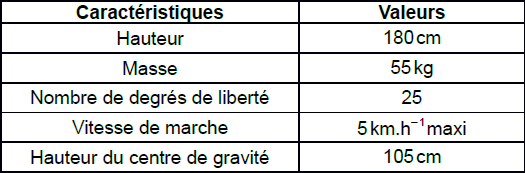
\includegraphics[width=\linewidth]{fig_01_a}
\end{center}

\subsection*{Contrôle de la posture de LOLA}
Pour assurer une marche rapide et stable de LOLA, la méthode choisie est le contrôle de la verticalité du tronc
du robot (figure 5). Le haut du corps (tronc, bras, tête) sera maintenu vertical en réalisant un asservissement
de position angulaire au niveau de l'articulation de la hanche. L'action mécanique de redressement est
développée par l'ensemble de motorisation de tangage autour de l'axe $(O_T,\vect{x_0})$. Les performances à vérifier
dans cette partie sont définies par les exigences suivantes.


\begin{center}
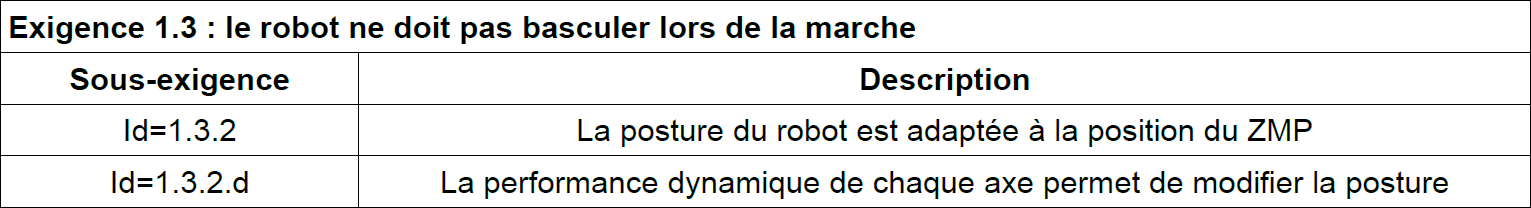
\includegraphics[width=\linewidth]{fig_05_a}
\end{center}


\begin{center}
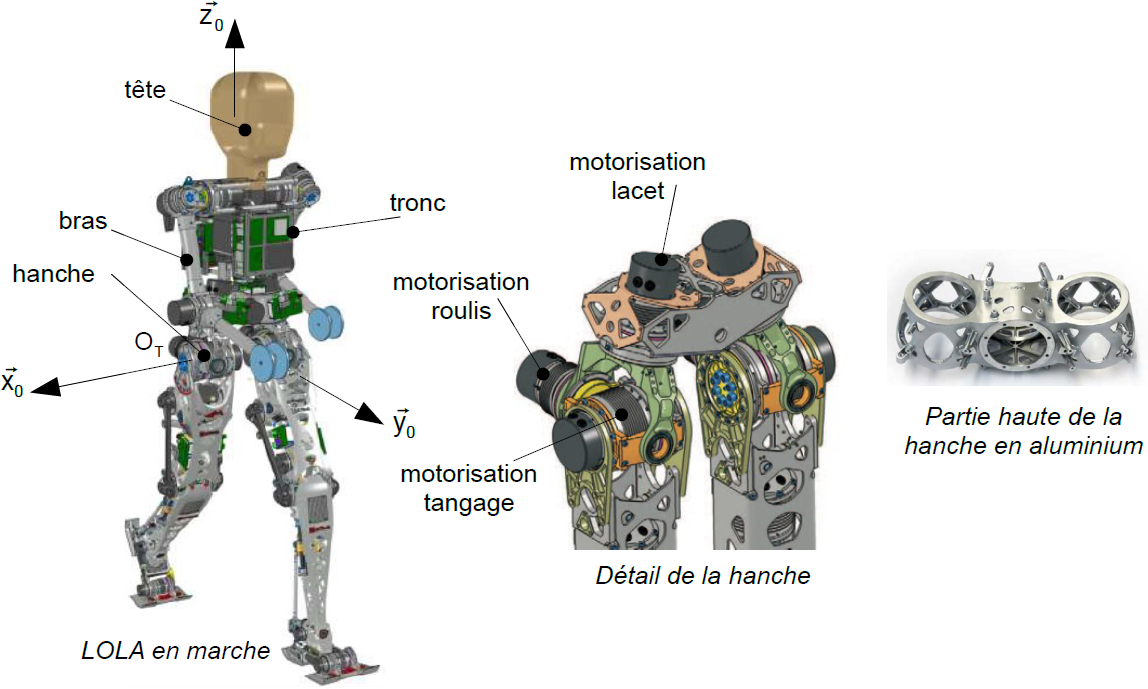
\includegraphics[width=\linewidth]{fig_05_b}
\end{center}

La chaîne structurelle permettant de modifier la posture du haut du corps autour de l'axe de tangage est
représentée sur la figure 6. Elle est composée d’un moteur électrique (1,2) synchrone à aimants
permanents piloté par un variateur électronique, d’un réducteur
Harmonic-Drive© (3) de rapport de réduction 1/100, d’un codeur
incrémental (5) ainsi que d’un codeur angulaire absolu (6+7).
Une centrale inertielle équipée d'un accéléromètre, d'un gyroscope et
d'une unité de traitement permet d'obtenir en temps réel la valeur de
l'angle d'inclinaison du haut du corps par rapport à la verticale.


\begin{center}
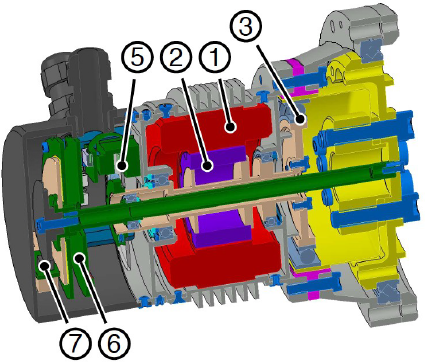
\includegraphics[width=.8\linewidth]{fig_06}
\end{center}

\fi

\begin{obj}
L'objectif de cette partie est de mettre en place un modèle du maintien
vertical du tronc de LOLA et de déterminer une structure de
commande permettant d'assurer les performances du cahier des
charges de l'exigence 1.3.2.
\end{obj}

\ifprof
\else
Les performances dynamiques de l'axe de tangage doivent vérifier les critères suivants:
\begin{center}
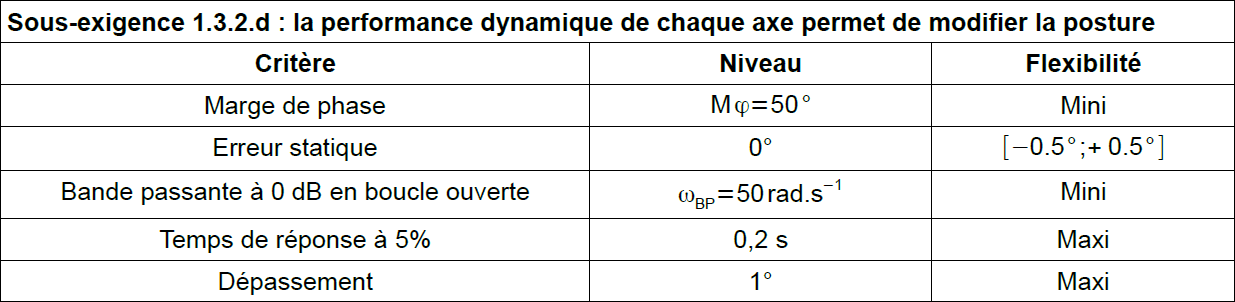
\includegraphics[width=\linewidth]{fig_07_a}
\end{center}
\fi
\subsection*{Modèle de connaissance de la dynamique de tangage}
\ifprof
\else
Le modèle mécanique utilisé pour mener notre étude est donné sur la figure suivante. L'association des liaisons entre
le tronc et les jambes au niveau de la hanche est équivalente, dans le plan sagittal $\left(O_T,\vect{y_0},\vect{z_0}\right)$, à une liaison pivot d'axe $\left(O_T,\vect{x_0}\right)$ . Le tronc sera considéré comme un solide admettant le plan $\left(O_T,\vect{y_0},\vect{z_0}\right)$ comme plan de
symétrie. Le cahier des charges stipule que LOLA doit pouvoir marcher à la vitesse de \SI{5}{km/h}. Cette vitesse
est atteinte en \SI{1}{s} lors de la première foulée. La loi de commande en vitesse correspondante est représentée
ci-dessous.

\begin{center}
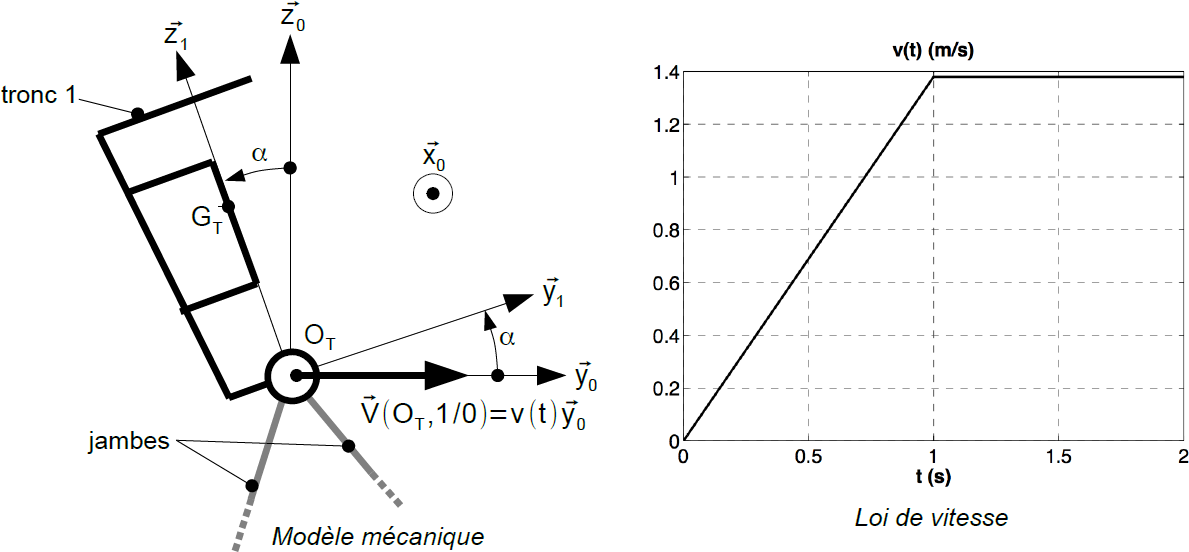
\includegraphics[width=\linewidth]{fig_07_b}
\end{center}

Le mouvement de marche est imposé et modélisé par le torseur cinématique en $O_T$ du mouvement du tronc 1
par rapport au sol 0 : $\torseurcin{V}{1}{0}=\torseurl{\dfrac{\dd \alpha}{\dd t}\vect{x_0}}{v(t)\vect{y_0}}{O_T}$.

Les caractéristiques d'inertie du tronc 1 de LOLA sont :
\begin{itemize}
\item la matrice d'inertie en $O_T$ $\inertie{O_T}{1} = \matinertie{A_1}{B_1}{C_1}{-D_1}{0}{0}{B_1}$;
\item position du centre de gravité : $\vect{O_TG_T}=Z_G\vect{z_1}$;
\item masse : $m_1$;
\item l'accélération de la pesanteur sera prise égale à $g=\SI{9,81}{m.s^{-2}}$ .
\end{itemize}


L'axe de sortie du réducteur exerce un couple de redressement sur le tronc 1 modélisé par le torseur couple
suivant : $\torseurstat{T}{\text{hd}}{1}=\torseurl{\vect{0}}{C_R\vect{x_0}}{O_T}$. L'angle $\alpha$ sera supposé faible pendant le mouvement : ainsi $\cos \alpha \simeq 1$ et $\sin \alpha \simeq \alpha$.

\fi
\subparagraph{} \textit{Proposer une démarche de résolution afin d'obtenir l'équation différentielle du mouvement reliant $\alpha$ et
ses dérivées successives aux données du problème. Effectuer un bilan des actions mécaniques
extérieures au système matériel isolé.}
\ifprof
\begin{corrige} ~\\

\begin{center}
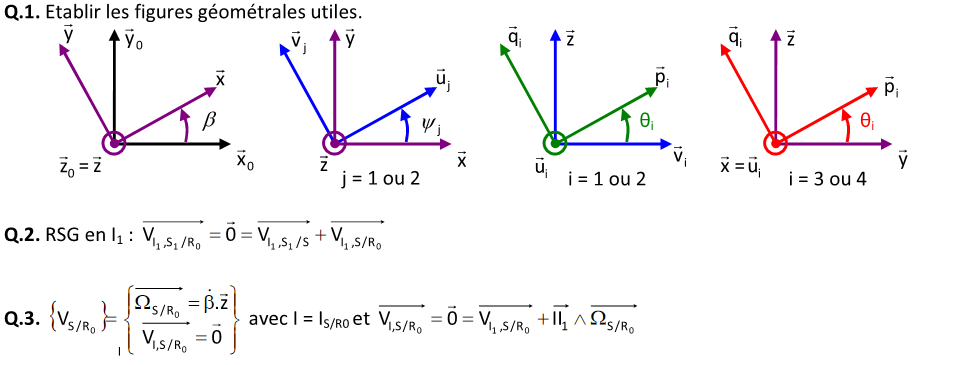
\includegraphics[width=.5\linewidth]{cor_01}
\end{center}

Pour ne pas faire apparaître des inconnues de liaisons, on va isoler 1 et réaliser un TMD en projection sur $\axe{O_T}{x_0}$.

Bilan des actions mécaniques extérieures à 1 : 
\begin{itemize}
\item action de la pesanteur;
\item $\torseurstat{T}{\text{hd}}{1}$;
\item action des jambes sur 1. 
\end{itemize}
\end{corrige}
\else
\fi


\subparagraph{} \textit{Développer l'ensemble des calculs pour déterminer l'équation différentielle reliant $\alpha$ et ses dérivées
successives aux données du problème.}
\ifprof
\begin{corrige} ~\\

\textbf{Déplacement du torseur de pesanteur}
On a : $\torseurstat{T}{\text{pes}}{1} = \torseurl{-gm_1\vect{z_0}}{\vect{0}}{G_T}$ 
%$= \torseurl{-gm_1\vect{z_0}}{\vect{O_TG}\wedge -gm_1\vect{z_0}}{O_T}$
$= \torseurl{-gm_1\vect{z_0}}{Z_G \vect{z_1}\wedge -gm_1\vect{z_0}}{O_T}$
$= \torseurl{-gm_1\vect{z_0}}{Z_G gm_1\sin\alpha \vect{x_0}}{O_T}$.


\textbf{Calcul du moment dynamique -- Formule point quelconque} 
\begin{itemize}
\item Calcul de $\vectv{G_T}{1}{0} =\vectv{O_T}{1}{0} + \vect{G_TO_T} \wedge \dot{\alpha} \vect{x_0}$
$=v(t)\vect{y_0}-Z_G\vect{z_1} \wedge \dot{\alpha}\vect{x_0}$
$=v(t)\vect{y_0}-Z_G \dot{\alpha}\vect{y_1}$.

\item Calcul de $\vectg{G_T}{1}{0} = \dot{v}(t)\vect{y_0} - Z_G \ddot{\alpha}\vect{y_1} -Z_G \dot{\alpha}^2\vect{z_1}$.

 \item  La matrice d'inertie est donnée en $O_T$, point quelconque. 

\item Commençons par calculer le moment cinétique : 
 
$\vectmc{1}{0}{O_T} = \inertie{O_T}{1}\vecto{1}{0}+m_1\vect{O_TG} \wedge \vectv{O_T}{1}{0}$
$=A_1\dot{\alpha}_1 \vect{x_1}  + m_1 Z_g\vect{z_1} \wedge v(t) \vect{y_0}$
$=A_1\dot{\alpha}_1 \vect{x_1}  - m_1 Z_g v(t)  \cos \alpha \vect{x_0}$ %\vect{z_1} \wedge  \vect{y_0}$


\item Calcul du moment dynamique :
  $\vectmd{1}{0}{O_T}=\left[\dfrac{\dd \vectmc{1}{0}{O_T}  }{\dd t }\right]_{\rep{0}} + m_1 \vectv{O_T}{1}{0}\wedge \vectv{G}{1}{0}$
$=A_1\ddot{\alpha}_1 \vect{x_1}  - m_1 Z_g \dot{v}(t)  \cos \alpha \vect{x_0} + m_1 Z_g v(t) \dot{\alpha} \sin \alpha \vect{x_0} + m_1 v(t) \vect{y_0}  \wedge \left(v(t)\vect{y_0}-Z_G \dot{\alpha}\vect{y_1}\right) $

$=A_1\ddot{\alpha}_1 \vect{x_1}  - m_1 Z_g \dot{v}(t)  \cos \alpha \vect{x_0} + m_1 Z_g v(t) \dot{\alpha} \sin \alpha \vect{x_0} -Z_G \dot{\alpha} m_1 v(t) \sin \alpha  \vect{x_0}  $
$=A_1\ddot{\alpha}_1 \vect{x_1}  - m_1 Z_g \dot{v}(t)  \cos \alpha \vect{x_0}  $

\end{itemize}
%
%
%$\vectmd{1}{0}{G} = \left[\dfrac{\dd \vectmc{1}{0}{G_T}}{\dd t}\right]_{\rep{0}}$ $=\left[\dfrac{\dd \left( A_1 \dot{\alpha}\vect{x_0}\right)}{\dd t}\right]_{\rep{0}}$
%$= A_1 \ddot{\alpha}\vect{x_0}$
%
%Déplacement en $O_T$. 
%
%On a $\vectmd{1}{0}{O_T} = \vectmd{1}{0}{G_T} + \vect{O_T G_T}\wedge m_1 \dot{v}(t) \vect{y_0}$
%$= A_1 \ddot{\alpha}\vect{x_0} + Z_G \vect{z_1} \wedge m_1 \dot{v}(t) \vect{y_0}$
%$= \left(A_1 \ddot{\alpha} - Z_G   m_1 \dot{v}(t) \cos \alpha \right)\vect{x_0} $.



\textbf{Calcul du moment dynamique -- Utilisation de Huygens} 
\begin{itemize}
\item Déplacement de la matrice d'inertie : $\vect{O_T G_T}=Z_G\vect{z_1}$. On a $\inertie{O_T}{1}=\inertie{G_T}{1}+m_1\begin{pmatrix}
Z_G^2 & 0 & 0 \\
0          & Z_G^2 & 0 \\
0 & 0 & 0 \\
\end{pmatrix}_{B_1}$. On a donc 
$\inertie{G}{1}
=\inertie{O_T}{1}-m_1\begin{pmatrix}
Z_G^2 & 0 & 0 \\
0          & Z_G^2 & 0 \\
0 & 0 & 0 \\
\end{pmatrix}_{B_1}
$  $ =\matinertie{A_1-m_1Z_G^2}{B_1-m_1Z_G^2}{C_1}{-D_1}{0}{0}{B_1}$
\item Calcul du moment cinétique : $\vectmc{G_T}{1}{0} = \inertie{G_T}{1} \vecto{1}{0}= \left( A_1-m_1Z_G^2 \right) \dot{\alpha} \vect{x_1}$.
\item Calcul du moment dynamique : $\vectmd{G_T}{1}{0} = \left( A_1-m_1Z_G^2 \right) \ddot{\alpha} \vect{x_1}$.
\item Déplacement du moment dynamique $\vectmd{O_T}{1}{0}=\vectmd{G_T}{1}{0}+ \vect{O_T G_T} \wedge  m_1\vectg{G_T}{1}{0} $ 

$=\vectmd{G_T}{1}{0}+m_1 \vect{O_T G_T} \wedge   \left(\dot{v}(t)\vect{y_0} - Z_G \ddot{\alpha}\vect{y_1} -Z_G \dot{\alpha}^2\vect{z_1} \right) $
$=\vectmd{G_T}{1}{0}+m_1 Z_G \vect{z_1} \wedge   \left(\dot{v}(t)\vect{y_0} - Z_G \ddot{\alpha}\vect{y_1} -Z_G \dot{\alpha}^2\vect{z_1} \right) $
$=\vectmd{G_T}{1}{0}+m_1 Z_G    \left(-\cos\alpha \dot{v}(t) \vect{x_0} + Z_G \ddot{\alpha}\vect{x_1}   \right) $

$= \left( A_1-m_1Z_G^2 \right) \ddot{\alpha} \vect{x_1}+m_1 Z_G    \left(-\cos\alpha \dot{v}(t) \vect{x_0} + Z_G \ddot{\alpha}\vect{x_1}   \right) $
$=  A_1\ddot{\alpha} \vect{x_1} - m_1 Z_G    \cos\alpha \dot{v}(t) \vect{x_0}     $
\end{itemize}

\textbf{Théorème du moment dynamique en $O_T$ suivant $\vect{x_0}$}

$A_1 \ddot{\alpha}(t) - Z_G   m_1 \dot{v}(t) \cos \alpha = Z_G gm_1\sin\alpha  +C_R $


\end{corrige}
\else
\fi

\ifprof
\else
Le contrôle de l'angle s'effectue par l'intermédiaire du moteur asservi en position, suivi du réducteur Harmonic-
Drive© de rapport de réduction $r= \dfrac{1}{100}$. Le moment d'inertie de l'arbre moteur suivant son axe de rotation est
noté $J_m$, le couple moteur exercé sur l'arbre d'entrée du réducteur est noté $C_m$. Le réducteur Harmonic-
Drive© sera considéré sans masse. La masse de l'arbre moteur est négligeable devant l'ensemble des autres
grandeurs inertielles. Une étude dynamique a permis de montrer que : $C_R=\dfrac{C_m}{r}-\dfrac{J_m}{r^2}\dfrac{\dd^2\alpha(t)}{\dd t^2}$. Ainsi, l'équation
différentielle du mouvement devient : 
$J_{\text{eq}} \dfrac{\dd^2\alpha(t)}{\dd t^2} -m_1gZ_G\alpha(t)=m_1 Z_G \dfrac{\dd v(t)}{\dd t}+\dfrac{C_m(t)}{r}$.

$J_{\text{eq}}$ est le moment d'inertie équivalent de l'ensemble du tronc ramené sur l'axe moteur.
\fi


\subsection*{Modèle du contrôle actif de la position verticale}
\ifprof
\else
On note $\Gamma(t)=\dfrac{\dd v(t)}{\dd t }$. Les conditions de Heaviside sont vérifiées. Le schéma-blocs du contrôle de la position angulaire du tronc de LOLA est représenté sur la figure suivante. La consigne angulaire est nulle afin de garder le
tronc du robot vertical: $\alpha_c(t)=0$. Les transformées de Laplace des fonctions seront notées en majuscules et
le paramètre de Laplace sera noté $p$.

\begin{center}
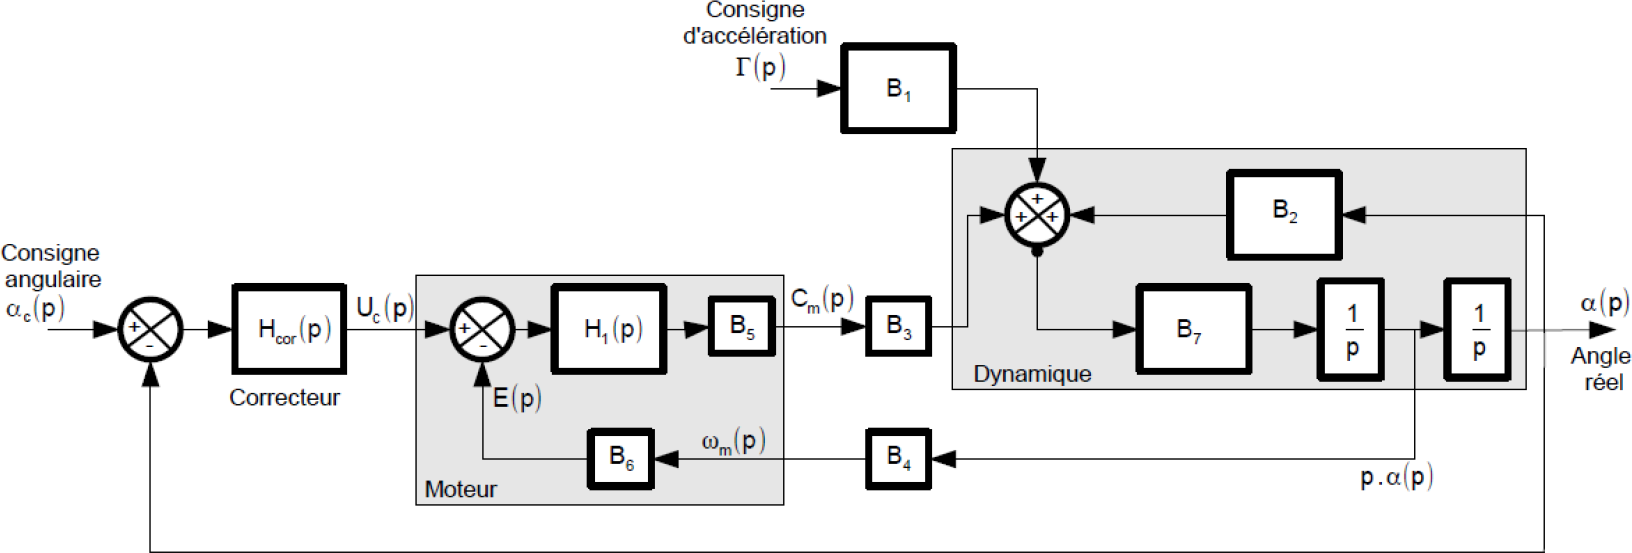
\includegraphics[width=\linewidth]{ann_02}
\end{center}



Le comportement du moteur sera considéré comme celui d'un moteur à courant continu dont les équations de
comportement sont les suivantes : $u_c (t)=e(t)+L \dfrac{\dd i(t)}{\dd t} +Ri (t)$; $e(t)=k_e\omega_m(t)$ et $C_m( t)=k_c i(t)$.

\fi

\subparagraph{} \textit{Indiquer les fonctions de transfert des blocs $B_1$, $B_2$, $B_3$, $B_4$ , $B_5$ , $B_6$ et $B_7$ ainsi que l'expression de la fonction de transfert $H_1(p)$ .}
\ifprof
\begin{corrige}
$B_6 = k_e$, $H_1(p)=\dfrac{1}{Lp + R}$, $B_5 = k_c$. 

On a de plus, $J_{\text{eq}} p^2 A(p) -m_1gZ_GA(p)=m_1 Z_G p V(p) +\dfrac{C_m(p)}{r}$.

On a donc $B_3 = \dfrac{1}{r}$, $p V(p) = \Gamma(p)$ et $B_1 = m_1 Z_G$, $B_2 =m_1gZ_G$ et $B_7 = \dfrac{1}{J_{\text{eq}}}$.

Enfin, $B_4 = \dfrac{1}{r}$.

\end{corrige}
\else
\fi

\ifprof
\else
Afin d'analyser la stabilité de cet asservissement, nous cherchons à déterminer la fonction de transfert en
boucle ouverte du système non-corrigé : $ F(p)= \dfrac{\alpha (p)}{U_c (p)}$ en supposant la perturbation nulle.
\fi

\subparagraph{} \textit{Déterminer la fonction de transfert de la boucle dynamique $H_{\text{dyn}}(p)=\dfrac{\alpha (p)}{C_m(p)}$ en supposant la perturbation nulle.}
\ifprof
\begin{corrige}
En déplaçant le point de prélèvement allant vers $B_2$ vers la gauche, $B_2$ est remplacé par $B_2/p$. On réduit donc la boucle (avec un + sur le retour) : $H_{\text{dyn}}(p)=\dfrac{\dfrac{B_7}{p}}{1-\dfrac{B_2B_7}{p^2}}\dfrac{B_3}{p}$ $=\dfrac{B_7}{1-\dfrac{B_2B_7}{p^2}}\dfrac{B_3}{p^2}$
 $=\dfrac{B_3B_7}{p^2-B_2B_7}$
  $=\dfrac{\dfrac{1}{r}\dfrac{1}{J_{\text{eq}}}}{p^2-m_1gZ_G\dfrac{1}{J_{\text{eq}}}}$
  
    $=\dfrac{1}{r J_{\text{eq}}p^2-m_1gZ_Gr}$.


\end{corrige}
\else
\fi


\subparagraph{} \textit{Déterminer la fonction de transfert en boucle ouverte non-corrigée de l'asservissement $ F(p)= \dfrac{\alpha (p)}{U_c (p)}$.
Indiquer son ordre, sa classe et donner son gain statique $K$ en fonction des données.}
\ifprof
\begin{corrige}

On réduit alors le bouclage sur le moteur : $F_2(p)=\dfrac{H_1B_5B_3 F(p)}{1+H_1B_5B_3 F(p)B_4 B_6}$. 

Au final, $H_{\text{dyn}}(p) = F_2 (p)\dfrac{1}{p}$ $=\dfrac{H_1B_5B_3 F(p)}{1+H_1B_5B_3 F(p)B_4 B_6} \cdot\dfrac{1}{p}$ $=\dfrac{H_1B_5B_3 \dfrac{B_7 p}{p^2-B_2B_7}}{1+H_1B_5B_3 \dfrac{B_7 p}{p^2-B_2B_7}B_4 B_6} \cdot\dfrac{1}{p}$

$=\dfrac{H_1B_5B_3 B_7 p}{\left(p^2-B_2B_7 \right)+H_1B_5B_3 B_7 pB_4 B_6} \cdot\dfrac{1}{p}$

$=\dfrac{\dfrac{1}{Lp + R}k_c\dfrac{1}{r} \dfrac{1}{J_{\text{eq}}} p}{\left(p^2-m_1gZ_G\dfrac{1}{J_{\text{eq}}} \right)+\dfrac{1}{Lp + R}k_c\dfrac{1}{r} \dfrac{1}{J_{\text{eq}}} p\dfrac{1}{r} k_e} \cdot\dfrac{1}{p}$

$=\dfrac{k_c }{ r J_{\text{eq}} \left(Lp + R\right) \left(p^2-m_1gZ_G\dfrac{1}{J_{\text{eq}}} \right)+k_c p\dfrac{1}{r} k_e} $


$=\dfrac{k_c }{ r J_{\text{eq}}  \left(Lp^3 + Rp^2-Lpm_1gZ_G\dfrac{1}{J_{\text{eq}}} - Rm_1gZ_G\dfrac{1}{J_{\text{eq}}} \right)+k_c p\dfrac{1}{r} k_e} $

$=\dfrac{k_c r}{   r^2 J_{\text{eq}}Lp^3 + r^2 J_{\text{eq}}Rp^2-r^2 Lpm_1gZ_G -r  Rm_1gZ_G +k_c p k_e} $

$=\dfrac{k_c r}{   r^2 J_{\text{eq}}Lp^3 + r^2 J_{\text{eq}}Rp^2+p\left(-r^2 Lm_1gZ_G  +k_c  k_e\right)-r  Rm_1gZ_G} $

$=\dfrac{\dfrac{k_c }{ Rm_1gZ_G}}{   \dfrac{r J_{\text{eq}}L}{ Rm_1gZ_G}p^3 + \dfrac{r J_{\text{eq}}}{  m_1gZ_G}p^2+p\dfrac{-r^2 Lm_1gZ_G  +k_c  k_e}{r  Rm_1gZ_G}-1} $.

Fonction de transfert d'ordre 3, de classe 0 et de gain $K=-\dfrac{k_c }{ Rm_1gZ_G}$.

\textbf{Erreur éventuelle avec des $r$ qui se baladent.}
\end{corrige}
\else
\fi

\ifprof
\else
Une simulation numérique permet de montrer que $F(p)$ est de la forme $\dfrac{K}{(1+ \tau_1p)(-1+ \tau_1p)(1+ \tau_2p)}$. Les diagrammes de Bode de cette fonction de transfert sont donnés ci-dessous.

\begin{center}
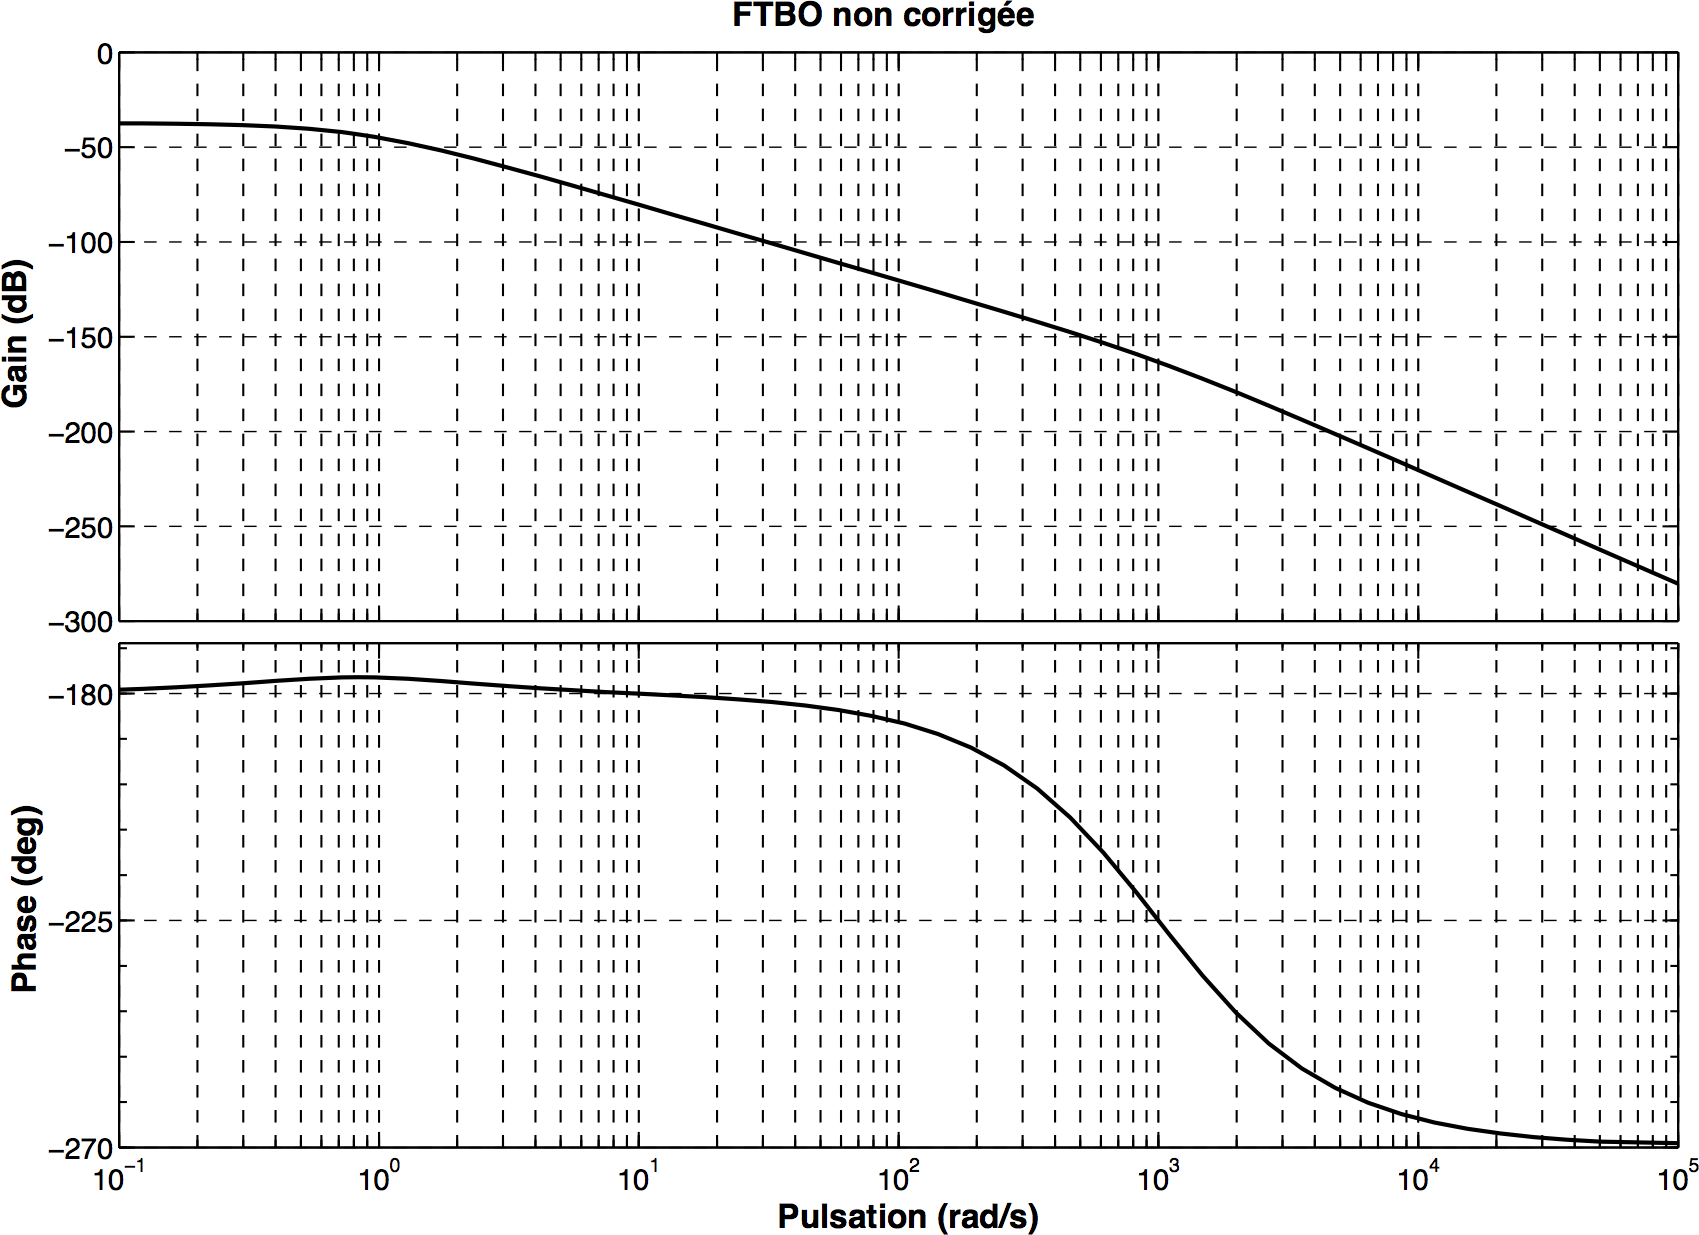
\includegraphics[width=\linewidth]{dr_12}
\end{center}
\fi


\subparagraph{} \textit{En analysant les diagrammes de Bode, déterminer les valeurs de $\tau_1$, $\tau_2$ et $K$. Justifier en complétant les diagrammes avec les diagrammes asymptotiques de
gain et de phase.}
\ifprof
\begin{corrige}
On a $G_{\text{dB}}(\omega)=20\log K - 20\log \sqrt{1+\tau_1^2\omega^2} - 20\log \sqrt{1+\tau_1^2\omega^2}-20\sqrt{1+\tau_2^2\omega^2}$ 

$=20\log K - 20\log \left(1+\tau_1^2\omega^2 \right)-20\log\sqrt{1+\tau_2^2\omega^2}$.


De plus $\varphi\left(\omega\right)=\arg K - \arg \left( 1+ \tau_1p\right)- \arg \left( -1+ \tau_1p\right)- \arg \left( 1+ \tau_2p\right)$ 

$= -\arctan\left( \tau_1 \omega\right)-\pi -\arctan\left( \tau_1 \omega\right)-\arctan\left( \tau_2 \omega\right)$

 $= -\pi-2\arctan\left( \tau_1 \omega\right)-\arctan\left( \tau_2 \omega\right)$.
 
 On a donc $\tau_1 = \dfrac{1}{\omega_1} = \SI{1}{s}$ et $\tau_2 = \dfrac{1}{\omega_2} = \SI{1e-3}{s}$.
 
 De plus, $20\log K=-40$ et $K=\SI{0,01}{rad.V^{-1}}$.
\end{corrige}
\else
\fi

\ifprof
\else
Pour la suite de l'étude, nous simplifierons $F(p)$ sous la forme suivante : $\dfrac{K}{(1+\tau_1p)(-1+ \tau_1p)}$.
\fi



\subparagraph{} \textit{Justifier le choix de cette simplification.}
\ifprof
\begin{corrige}
Les pôles de la fonction de transfert sont $\dfrac{-1}{\tau_1}=-1$, $\dfrac{1}{\tau_1}=1$ et $\dfrac{-1}{\tau_2}=-1000$. Les poles dominants sont ceux les plus proches de l'axe des imaginaires. $-1$ et $1$ sont donc les pôles dominants. Cela justifie donc la forme proposée (le pôle $-1000$ est négligé).
\end{corrige}
\else
\fi


\subparagraph{} \textit{Expliquer pourquoi le critère du revers ne peut pas être appliqué pour étudier la stabilité en boucle
fermée.}
\ifprof
\begin{corrige}
Pour que le critère du revers, les pôles doivent être à partie réelle négative ou nulle. 
\end{corrige}
\else
\fi


\ifprof
\else
Afin de résoudre ce problème, il est décidé d'asservir la chaîne directe en position et en vitesse. Pour cela, la centrale inertielle permet de mesurer l'angle de tangage $\alpha (t )$ ainsi que la vitesse angulaire $\dfrac{\dd \alpha(t)}{\dd t}$.

L'asservissement ainsi réalisé est présenté sous la forme du schéma-blocs de la figure suivante.
$U_c (p)$ est la tension de commande en sortie du correcteur. La fonction de transfert de la centrale inertielle
sera prise égale à $H_{\text{c i}}(p)=K_1(p+1)$.

\begin{center}
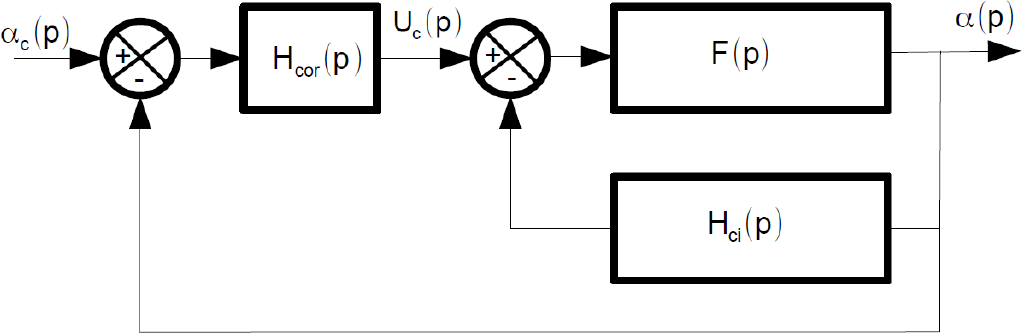
\includegraphics[width=\linewidth]{fig_08}
\end{center}
\fi


\subparagraph{} \textit{Déterminer deux conditions sur $K_1$ pour que la fonction de transfert en boucle ouverte non-corrigée $\dfrac{\alpha (p)}{U_C(p)}$ soit stable. En déduire la valeur minimale de $K_1$.}
\ifprof
\begin{corrige}
La fonction de transfert en boucle ouverte non corrigée est donnée par : $\dfrac{F(p)}{1+F(p)H_{\text{c i}}(p)}$ 

$=\dfrac{\dfrac{K}{(1+\tau_1p)(-1+ \tau_1p)}}{1+\dfrac{K}{(1+\tau_1p)(-1+ \tau_1p)} K_1(p+1) }$
$=\dfrac{K}{(1+\tau_1p)(-1+ \tau_1p)+K K_1(p+1) }$
$=\dfrac{K}{-1-\tau_1p+\tau_1p + \tau_1^2p^2+K K_1p+K K_1 }$
$=\dfrac{K}{-1+K K_1  +K K_1p + \tau_1^2p^2}$. Il faut donc que $KK_1 -1>0$ soit $K_1 >\dfrac{1}{K}$ soit $K_1>\SI{100}{V.rad^{-1}}$.
\end{corrige}
\else
\fi



\subparagraph{} \textit{Déterminer $K_1$ pour que la fonction de transfert $\dfrac{\alpha (p)}{U_C(p)}$
 ait un facteur d'amortissement $\xi=1,7$.
Vérifier que cette valeur est compatible avec les conditions obtenues précédemment. En déduire les
valeurs de la pulsation propre $\omega_0$ et du gain statique de la boucle ouverte $K_{\text{BO}}$.}
\ifprof
\begin{corrige}~\\

En mettant la fonction précédente sous forme canonique, on a donc $\dfrac{\dfrac{K}{K K_1-1}}{ 1 +\dfrac{K K_1}{K K_1-1}p + \dfrac{\tau_1^2}{K K_1-1}p^2}$.

On a $\dfrac{1}{\omega_0^2}= \dfrac{\tau_1^2}{K K_1-1}$ $\Leftrightarrow {\omega_0^2}= \dfrac{K K_1-1}{\tau_1^2}$. 

De plus, $\dfrac{2\xi}{\omega_0} = \dfrac{K K_1}{K K_1-1}$ $\Leftrightarrow 2\xi \left( K K_1-1 \right) = K K_1 \omega_0$  $\Leftrightarrow 2\xi \left( K K_1-1 \right) = K K_1 \sqrt{K K_1-1}$.

 $\Rightarrow 4\xi^2 \left( K K_1-1 \right)^2 = K^2 K_1^2 \left(K K_1-1\right)$
  $\Leftrightarrow 4\xi^2 \left( K K_1-1 \right)^2 - K^2 K_1^2 \left(K K_1-1\right)=0$
    $\Leftrightarrow 4\xi^2 \left( K K_1-1 \right) - K^2 K_1^2 =0$
\end{corrige}
\else
\fi

\ifprof
\else
Quels que soient les résultats trouvés précédemment, nous utiliserons les expressions suivantes pour la suite
de l'étude : $\dfrac{\alpha (p)}{U_C(p)} = \dfrac{K_{\text{BO}}}{1+\dfrac{2\xi}{\omega_0}p+\dfrac{p^2}{\omega_0^2}}$
avec $K_{\text{BO}}=1,1\cdot 10^{-3}$, $\xi=1,7$ et $\omega_0=\SI{3}{rad.s^{-1}}$ . Pour répondre au cahier des
charges, il est décidé d'implanter un correcteur de fonction de transfert suivante : $H_{\text{cor}} (p)=K_p \dfrac{1+aT_d p}{1+T_d p}$ avec $a>1$.

\fi

\subparagraph{} \textit{Nommer ce correcteur.}
\ifprof
\begin{corrige}
Il s'agit d'un correcteur proportionnel et à avance de phase. 
\end{corrige}
\else
\fi

\ifprof
\else
Les diagrammes de Bode de gain et de phase (pour $K_p=1$ ) de ce correcteur sont fournis ci-dessous. Afin
d'assurer un gain significatif de phase, nous décidons de placer $\omega_c$ en $\omega_{\text{BP}}=\SI{50}{rad.s^{-1}}$, définissant ainsi la bande passante.

\begin{center}
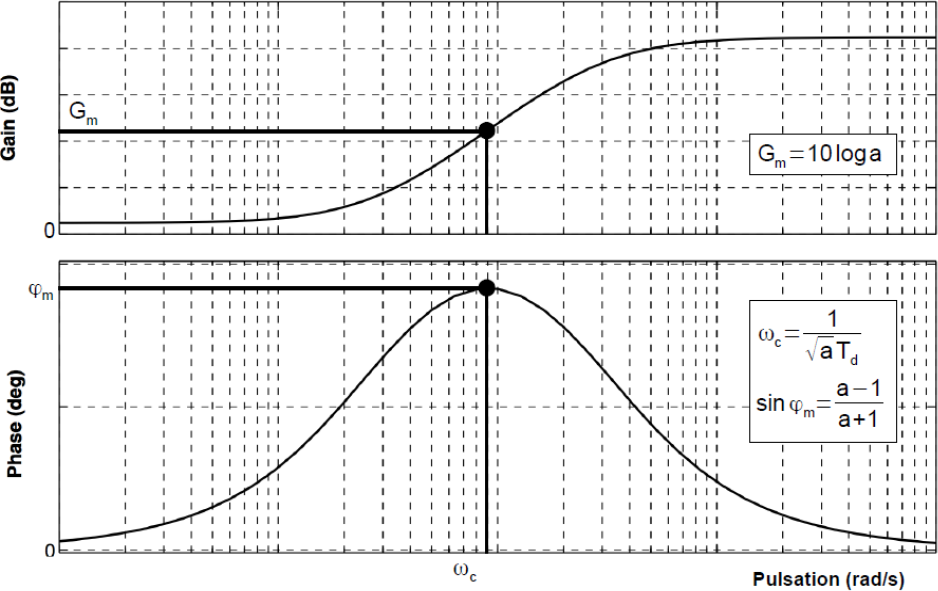
\includegraphics[width=\linewidth]{ann_03}
\end{center}

\fi

\subparagraph{} \textit{Déterminer la valeur du paramètre a pour que le correcteur permette d'assurer la marge de phase
du cahier des charges. En déduire la valeur de $T_d$.}
\ifprof
\begin{corrige} ~\\

D'après le cahier des charges, on souhaite que la bande passante à \SI{0}{dB} en boucle ouverte soit de \SI{50}{rad.s^{-1}} et la marge de phase doit être de 50\degres.

\textbf{Calculons la phase pour le système non corrigé.}

Pour calculer la phase, il faut faire attention, au domaine de définition de l'arctan. Il y a plusieurs façons de s'y prendre...
On peut par exemple calculer les deux constantes de temps du système (vu que $\xi>1$). On peut aussi constater que pour un second ordre où $\xi>1$, la phase est comprise entre 0 et $-90\degres$ lorsque la pulsation est inférieure à \SI{3}{rad.s^{-1}} et la phase est comprise entre $-90$ et $-180\degres$ lorsque la pulsation est supérieure à \SI{3}{rad.s^{-1}}. 

Ici on souhaite calculer la marge pour une pulsation de \SI{50}{rad.s^{-1}}. On aura donc une phase comprise entre $-90$ et $-180\degres$. Le calcul de l'arctan se fera donc avec un décalage de $-180\degres$. 



$\varphi\left(\omega\right)=-180- \arctan\left( \dfrac{\dfrac{2 \xi \omega}{\omega_0}}{1-\dfrac{\omega^2}{\omega_0^2}}\right)=-168\degres $.

La marge de phase est donc de $-168-(-180) = 12\degres$. Le correcteur doit donc apporter 38\degres. 

On a $\sin\varphi_m = \dfrac{a-1}{a+1}$ $\Leftrightarrow a \sin\varphi_m + \sin\varphi_m = a- 1 $
$\Leftrightarrow a \sin\varphi_m + \sin\varphi_m -a+1 = 0 $

$\Leftrightarrow a \left( \sin\varphi_m -1\right)+ \sin\varphi_m +1 = 0 $
$\Leftrightarrow a   = \dfrac{\sin\varphi_m +1}{1-\sin\varphi_m} =4,28$.

Par suite, $T_d = \dfrac{1}{\omega_c\sqrt{a}}\simeq \SI{9,7e-3}{s}$.


%Tout d'abord, $\xi>1$. On peut donc factoriser le dénominateur. 
%On a $\Delta = \dfrac{4\xi^2}{\omega_0^2}-\dfrac{4}{\omega_0^2}=\dfrac{4}{\omega_0^2}\left(\xi^2 - 1 \right) = \left(\dfrac{2}{\omega_0}\sqrt{\xi^2 - 1}\right)^2$.
%On a donc $p_{1,2} = \dfrac{- \dfrac{2\xi }{\omega_0}\pm\left(\dfrac{2}{\omega_0}\sqrt{\xi^2 - 1}\right) }{\dfrac{2}{\omega_0^2}}$ 
%$= \omega_0\left(- \xi\pm\sqrt{\xi^2 - 1} \right)$.
%
%Le dénominateur est donc de la forme $\dfrac{1}{\omega_0^2}\left( p-  \omega_0\left(- \xi-\sqrt{\xi^2 - 1} \right)\right)\left( p-  \omega_0\left(- \xi+\sqrt{\xi^2 - 1} \right)\right)$
%
% $=\dfrac{1}{\omega_0^2}\left( p+ \omega_0\left( \xi+\sqrt{\xi^2 - 1} \right)\right)\left( p+  \omega_0\left(\xi-\sqrt{\xi^2 - 1} \right)\right)$. 
 

\end{corrige}
\else
\fi


\subparagraph{} \textit{Déterminer le gain $K_p$ pour que le critère de bande passante du cahier des charges soit bien vérifié.}
\ifprof
\begin{corrige}
On doit choisir $K_p$ pour que le gain soit nul lorsque $\omega_c = \SI{50}{rad.s^{-1}}$. 

La gain non corrigé est de $G_{\text{dB}}(\omega)=20\log K_{BO} - 20 \log \left( \sqrt{\left( 1-\dfrac{\omega^2}{\omega_0^2}\right)^2+\left( \dfrac{2\omega\xi}{\omega_0}\right)^2}\right)$
$=\SI{-108}{dB}$.

Le gain apporté par l'avance de phase est de $10\log a=\SI{6,31}{dB}$. Le gain proportionnel doit donc apporter $-108+6=\SI{102}{dB}$. On cherche donc $20\log K_p = 102$ soit $K_p = 10^{102/20}=\SI{125892}{SI}$
\end{corrige}
\else
\fi
\ifprof
\else
La stabilité du tronc étant assurée, nous devons maintenant analyser les performances en précision et rapidité
de l'asservissement de position angulaire. La consigne est nulle, ainsi seule la perturbation va écarter le tronc
du robot de sa posture verticale. Cette perturbation provient du mouvement de marche souhaité c'est à dire de
l'accélération subie $\Gamma(t)=\dfrac{\dd v(t)}{\dd t}$. Avec les réglages du correcteur, une simulation numérique a permis de tracer la réponse temporelle du système pour une perturbation $\Gamma(t)$ respectant la loi de vitesse présentée précédemment.
Cette réponse est tracée sur la figure suivante.

\begin{center}
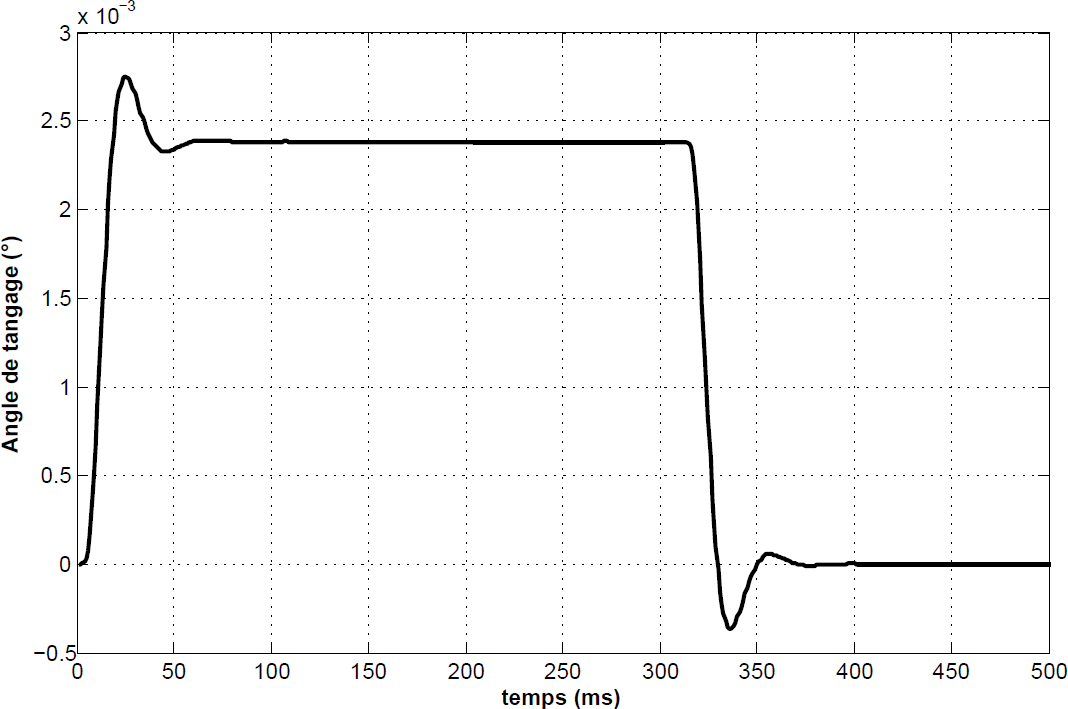
\includegraphics[width=\linewidth]{ann_04}
\end{center}
\fi


\subparagraph{} \textit{Justifier l'allure de la réponse temporelle. Déterminer graphiquement sur le document réponse le temps de réponse à 5\%, le dépassement maximal et l'erreur statique. Conclure sur la capacité du correcteur à
vérifier l'ensemble des critères du cahier des charges.}
\ifprof
\begin{corrige}
Le système est perturbé << en accélération >>. On souhaite minimiser l'influence de cette perturbation sur l'angle de tangage (souhaité nul).
On mesure : 
\begin{itemize}
\item temps de réponse à 5\% : $\SI{40}{ms} <\SI{0,2}{s}$ : CDCF OK;
\item écart statique : $\simeq \SI{2,4e3}{\degres} <0,5\degres$ : CDCF OK;
\item dépassement $\simeq \SI{0,8e3}{\degres} <1\degres$ : CDCF OK.
\end{itemize}
\end{corrige}
\else
\fi



\ifprof
\else
\end{multicols}
\fi

